\documentclass{article}
\usepackage[spanish]{babel}
\usepackage[utf8]{inputenc}
\usepackage{graphicx}
\usepackage{fancyhdr}
\usepackage{amssymb,amsmath,amsthm}
\usepackage{geometry}
\usepackage{enumerate}

%Comandos:
\newcommand{\R}{\mathbb{R}}
\newcommand{\N}{\mathbb{N}}

% Configuración de página:
\geometry{letterpaper,margin=2cm,tmargin=3cm}

\fancypagestyle{plain}{
	\fancyhead[L]{Universidad de Chile\\Facultad de Ciencias Físicas y Matemáticas\\MDS7203 Modelos Generativos Profundos}
	\fancyhead[R]{
\includegraphics[height=1.5cm]{images/fcfm}}
}
\pagestyle{fancy}{
\fancyhead[L]{Facultad de Ciencias Físicas y Matemáticas}
\fancyhead[R]{Universidad de Chile}
}

%Título:
\title{\bfseries{Control de Lectura nº1}\vspace{0.5cm}}
\author{\textbf{Nombre:} \rule{12cm}{0.4pt}}

% Documento:
\begin{document}
\maketitle

\hspace{-0.5cm}\textbf{Instrucciones:} Responda las siguientes preguntas de forma breve y concisa. El control de lectura tiene una duración de 15 minutos y no está permitido el uso de apuntes ni dispositivos electrónicos.

\section*{Redes bayesianas}
\begin{enumerate}[{\bf P1.}]
	\item ¿Cómo factoriza la distribución conjunta $p(x_1,\ldots,x_6)$ la red bayesiana asociada al siguiente DAG?
	      \begin{figure}[h]
		      \centering
		      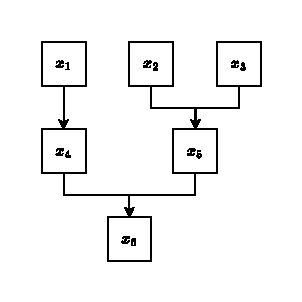
\includegraphics[width=0.3\textwidth]{images/dag.pdf}
	      \end{figure}
	\item ¿Cómo se genera una muestra $x\sim p(x)$ a partir de un modelo de variable latente $p(x,z)=p(z)p(x|z)$?
\end{enumerate}

\section*{Modelos autorregresivos}
\begin{enumerate}[{\bf P1.}]
	\item Nombre 3 tokens especiales usados al modelar secuencias de texto, e indique su función.
	\item ¿En qué consiste la técnica de temperatura usada en la generación de texto?
\end{enumerate}

\end{document}